\graphicspath{{./images/}}

\newcounter{nonFuncReq} %Non functinal requiremet counter
\newcounter{quatar} %Quality target counter

\chapter{Einführung und Ziele}

\section{Business Case}
\label{businesscase}

Die Applikation MEON (Merchant Onboarding) dient der Registration neuer Händler für den mobilen Bezahldienst TWINT und zukünftig der Registrierung neuer Händler für Enabling(Terminal)/Acquiring Pakete. Der Geschäftsprozess läuft in zwei Teilen ab welche durch verschiedene Teile der Applikation durchgeführt werden.  Dabei soll es einem Händler möglich sein, sich ohne direkten Kontakt mit der SIX einen gültigen Vertrag für den Einsatz des Dienstes zu erwerben. Sollte ein Kontakt notwendig sein, wird dieser seitens SIX durch das Risk Management initiiert.\newline
Die Anwendung soll eine moderne und intuitive Web Applikation sein und dem Benutzer möglichst viele Hilfestellung bieten. Nach der erfolgreichen Registrierung und  eventuellen Prüfung soll der Dienst auf den notwendigen internen System der SIX automatisch aufgeschaltet werden. Hierzu zählen das System für die Verwaltung der Terminals (SCS) sowie das Transaktionsverarbeitungsystem(PASS).

\begin{figure}[H]
	\centering
	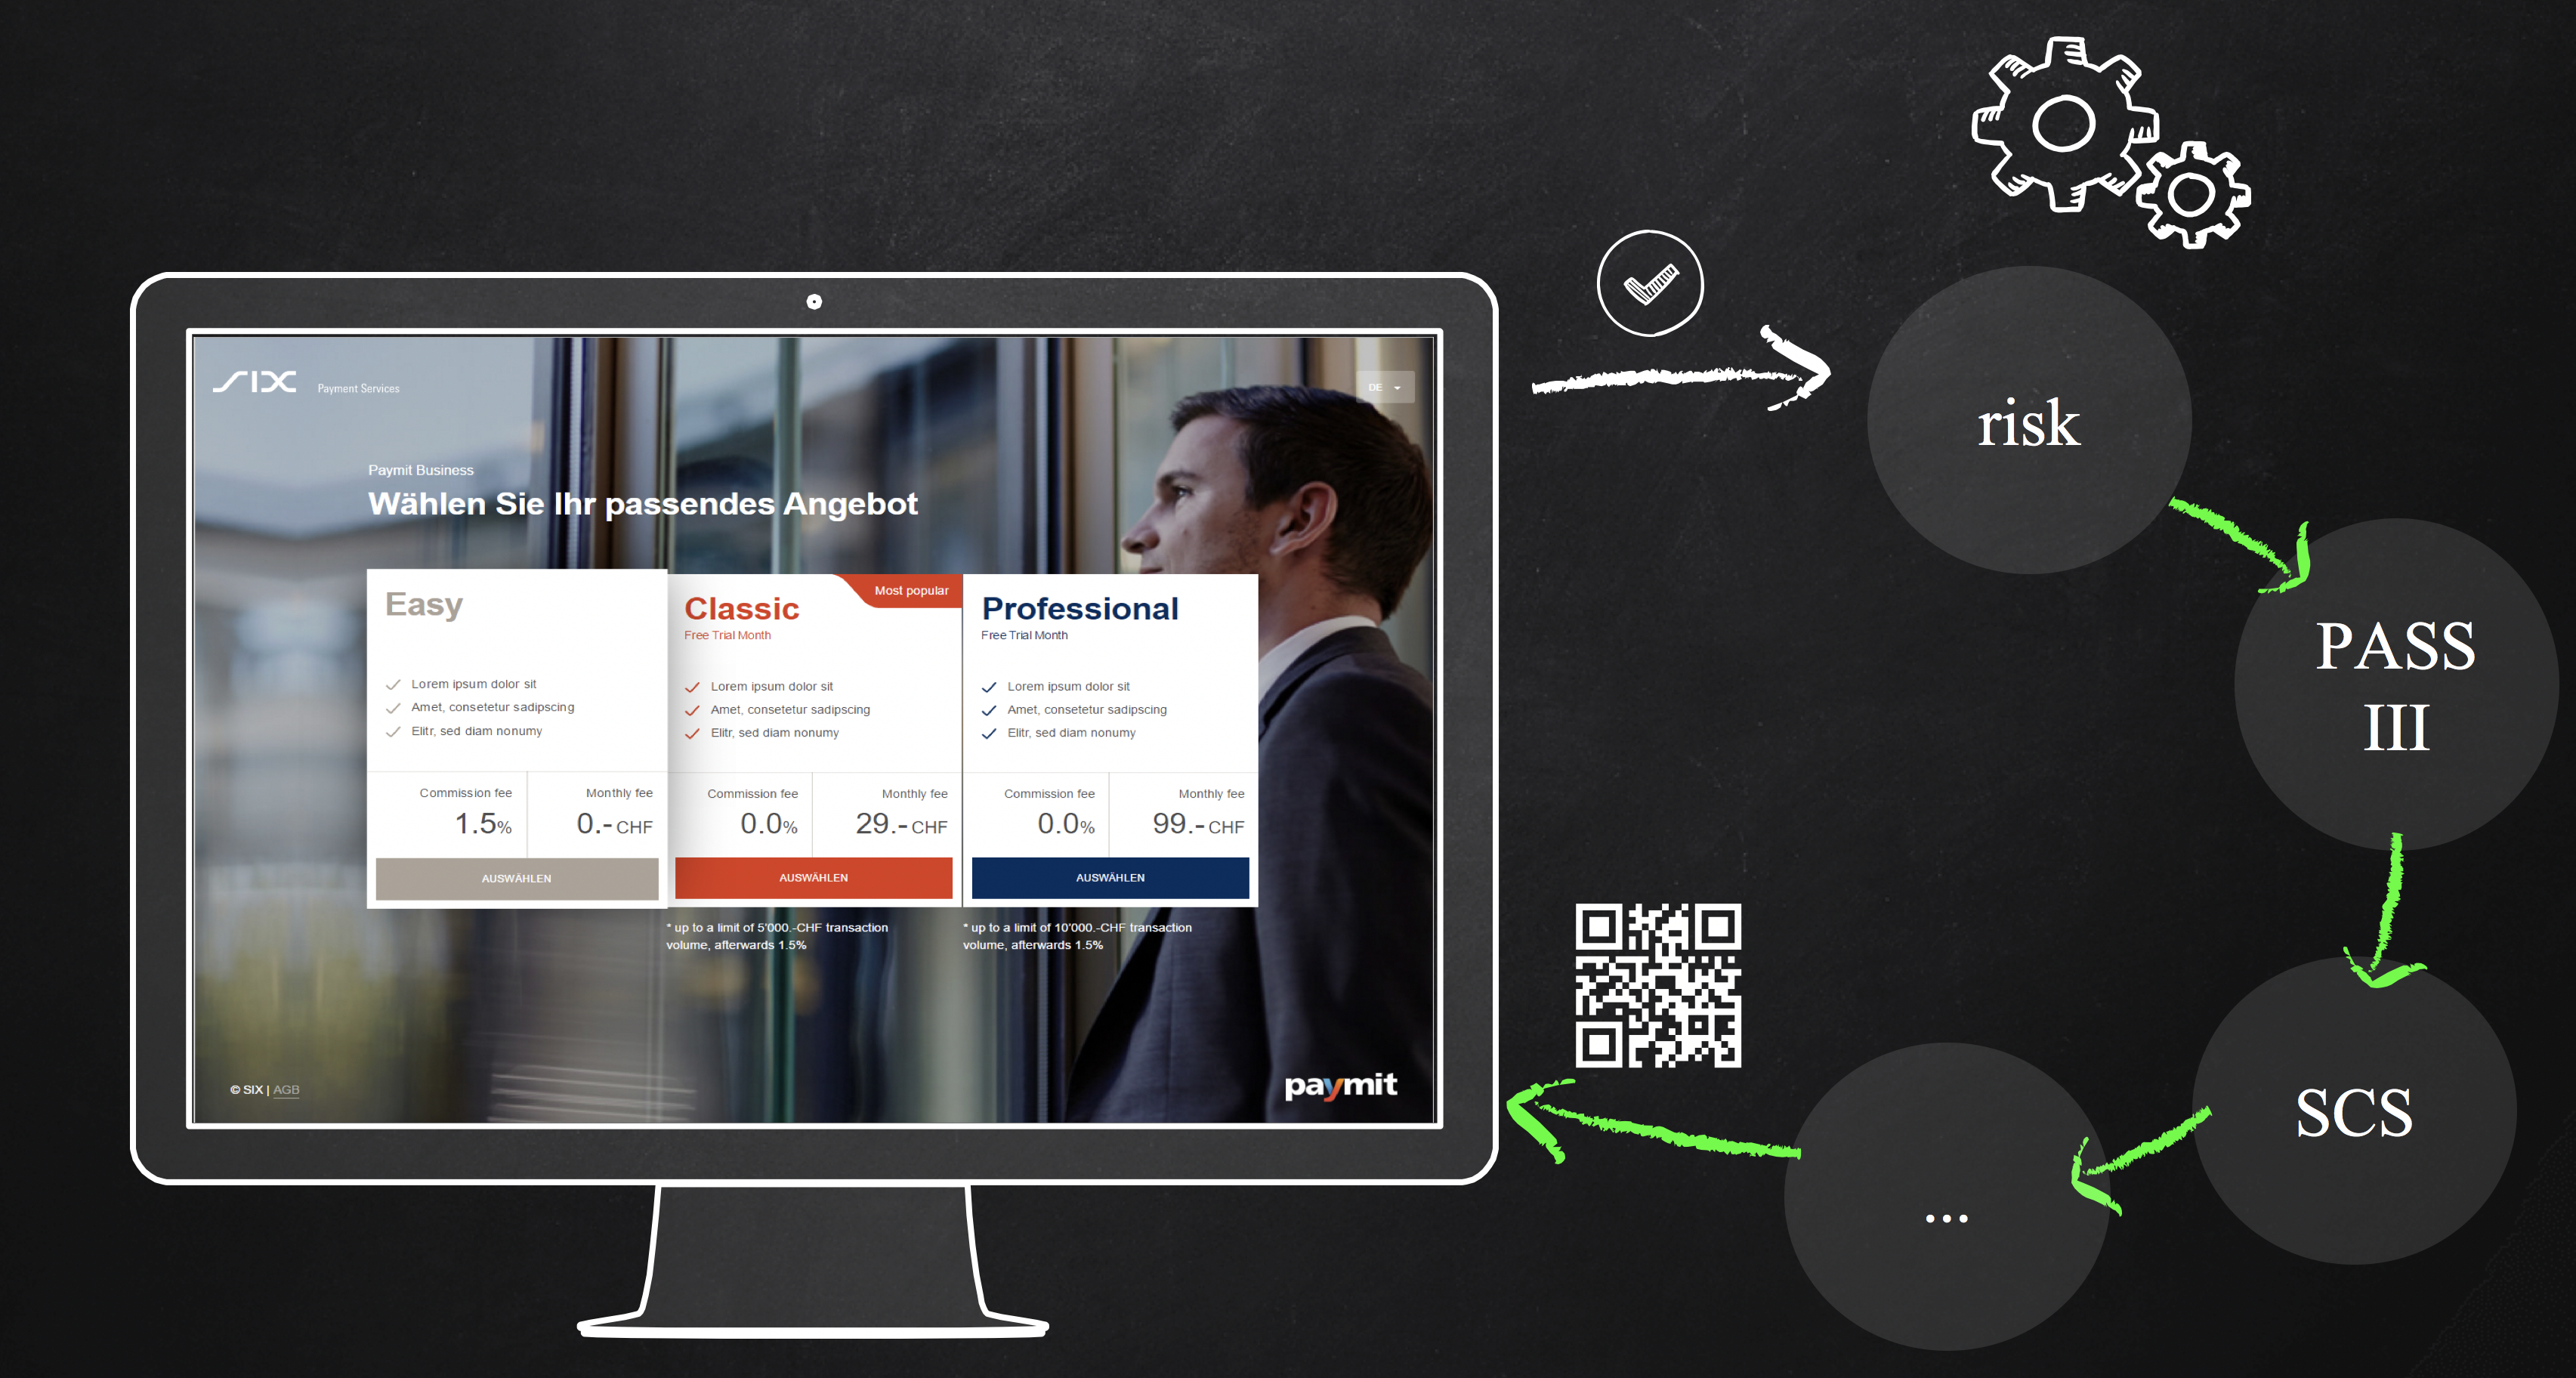
\includegraphics[scale=0.25]{meon-use-case.png}
	\caption{MEON Business Case}
\end{figure}
\newpage
\section{Aufgabenstellung}

Die neue Architektur der Applikation soll die unterbrechungsfrei Installation des Onboarding Servers erlauben(Continuous Deployment). Da die Anwendung bereits in Betrieb ist, sollen Änderungen nur gemacht werden, wenn sie für die Umsetzung unumgänglich sind. \newline Die Workflow Engines ist ein Produkt der Firma Camuda. Diese wird jedoch in der Open Source version verwendet. Das Produkt hat bereits Mechanismen für Continuous Deployment, SIX besitzt zur Zeit aber keinen Supportvertag um diese Feature in Betrieb zunehmen. Aus diesem Grund wird die Engine nicht in die Architektur aufgenommen was für den  Onboarding Server bedeutet, dass dieser Umstand berücksichtigen werden muss um die Anforderungen zu erfüllen.

\section{Anforderungen}
\label{requirements}
Alle funktionalen Anforderungen sind bereits umgesetzt. Durch die Anpassung der Architektur in Richtung Continuous Deployment gibt es aktuell nur nicht funktionale Anforderungen.

\stepcounter{nonFuncReq}
\begin{table}[H]
	\centering
	\caption{Nicht funktionale Anforderungen}
	\begin{tabular}{ | p{2cm} | p{13cm} | }
		\toprule
		\textbf{ID} & \textbf{Beschreibung} \\
		\midrule
		NFA-\arabic{nonFuncReq} \stepcounter{nonFuncReq} & Kunde merkt nicht wenn neue Komponenten der Applikation ausgetauscht werden. \\ \hline
		NFA-\arabic{nonFuncReq} \stepcounter{nonFuncReq} & Verfügbarkeit der Frontend-Anwendung ist 24x7 (SLA). \\ \hline
		NFA-\arabic{nonFuncReq} \stepcounter{nonFuncReq} & Einhaltung der PCI DSS Anforderung bezüglich Umgang mit Daten resp. deren Zugriffsschutz durch Authentifizierung, Autorisierung und Netzwerksegmentierung. \\ \hline
		NFA-\arabic{nonFuncReq} \stepcounter{nonFuncReq} & Die Applikation muss horizontal skalierbar sein. \\ \hline
		NFA-\arabic{nonFuncReq} \stepcounter{nonFuncReq} & Die Anwendung muss eine hohe Ausfallsicherheit für Server und die Datenbank aufweisen. \\ \hline
		NFA-\arabic{nonFuncReq} \stepcounter{nonFuncReq} & Bugfixing geschieht mittels vorwärts committen, anstelle von Hotfixes wird immer die ganze Applikation neu ausgerollt. \\ \hline
		NFA-\arabic{nonFuncReq} \stepcounter{nonFuncReq} & Die Anwendung lässt sich voll automatisch Ausrollen. \\ \hline
		NFA-\arabic{nonFuncReq} \stepcounter{nonFuncReq} & Konfigurationsänderungen an der Applikation sind ohne Neustart möglich.\\
		\bottomrule
	\end{tabular}
\end{table}

\subsection{Kernaufgabe}

Ziel ist die Akquirierung neuer Händler für das mobile Bezahlsystem TWINT.

\subsection{Art des Systems}

Die Applikation MEON besteht aus zwei Teilen. Der Onboarding Server ist ein interaktives Online System, die Workflow Engines ist ein Hintergrundsystem.

\subsection{Datenhaltung}

Die Datenhaltung wird mittels MongoDB für den Onboarding Server und Oracle für die Workflow Engine sichergestellt.

\subsection{Schnittstellen}

MEON hat folgende Schnittstellen zu Umsystemen welche lesend(ro) oder schreiben(w) sein können.
\begin{itemize}
	\item AddressService: Adressen Service der Post (ro)
	\item UID: Schweizer Unternehmens-Identifikationsnummer (ro) 
	\item ZEFIX: Handelsregisteranbindung (ro)
	\item ATMS: SMS Service (w)
	\item Email: Email Service (w)
	\item Workflow: Workflow Engine Backoffice SIX (w)
\end{itemize}

\section{Qualitätsziele}

Die folgende Tabelle zeigt die wichtigsten Qualitätsziele. Die Szenarien zu den Zielen sind genauer im Kapitel \ref{sec:qualityscenarios} aufgeführt.

\stepcounter{quatar} 
\begin{table}[H]
	\centering
	\caption{Qualitätsziele}
	\begin{tabular}{ | p{1cm} | p{11cm} | p{3cm} | }
		\toprule
		{\textbf{ID}} & {\textbf{Beschreibung}} & {\textbf{Anforderung}}\\
		\midrule
		Q-\arabic{quatar} \stepcounter{quatar} & Der Zugriff auf sensitive Daten (PCI) darf nicht möglich sein. & NFA-3\\ \hline
		Q-\arabic{quatar} \stepcounter{quatar} & Anpassungen an der Software sollen schnell eingeführt werden können. & NFA-6, NFA-7\\ \hline
		Q-\arabic{quatar} \stepcounter{quatar} & Die Applikation soll ohne Unterbrechung des Dienstes installiert werden können. & NFA-1\\ \hline
		Q-\arabic{quatar} \stepcounter{quatar} & Der Händler soll sich, bei korrektem Ausfüllen der Daten, registrieren können. & NFA-2, NFA-5 \\ \hline
		Q-\arabic{quatar} \stepcounter{quatar} & Konfigurationsänderungen an der Applikation können ohne Unterbruch durchgeführt werden. & NFA-8 \\ \hline
		Q-\arabic{quatar} \stepcounter{quatar} & Die Applikation soll schnell horizontal skaliert werden können. & NFA-4 \\
		\bottomrule
	\end{tabular}
\end{table}

\section{Stakeholder}

\begin{table}[H]
	\centering
	\caption{Stakeholder}
	\begin{tabular}{ | p{3cm} | p{12cm} | }
		\toprule
		{\textbf{Name}} & {\textbf{Beschreibung}} \\
		\midrule
		Business & Repräsentiert die Geschäftstätigkeit der Firma.\\ \hline
		Kunde & Benutzer der Webapplikation. \\ \hline
		Support-Kunde & Support welcher den Kunden bei Problemen unterstützt. \\ \hline
		Legal &  Verantwortlich für die Richtigkeit der Vertragsabschlüsse. \\ \hline
		Risk & Sorgt für die Überprüfung der Personen und der Geschäftstätigkeiten. \\ \hline
		Marketing & Abteilung für den Vertrieb, Werbung, Design. \\ \hline
		Betrieb & Betreibt die Webapplikation auf der Infrastruktur der SIX \\ \hline
		Change Management & Genehmigt Änderungen an der Applikation. \\ \hline
		Entwickler & Setzt die Anforderungen der einzelnen Stakeholder um. \\
		\bottomrule
	\end{tabular}
\end{table}
